\subsection {Number of comments by a specific user}\label{subsec:comments-by-user}
    \begin{verbatim}
        SELECT COUNT(*)
          FROM   schema.comments_constrained
          WHERE  author='username';
    \end{verbatim}
    All usernames can be queried from the schema.redditors table.
    Showing one example of running this code as a stored function in figure~\ref{fig:number-of-comments-figure} below.
    \begin{figure}[h]
    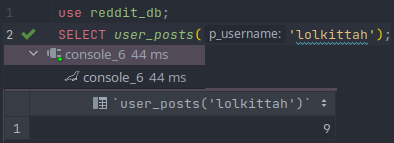
\includegraphics[width=400px] {number_of_posts}\label{fig:number-of-comments-figure}
        \caption {The query was run in about 44ms}
    \end{figure}

\subsection{Comments per day in subreddit}\label{subsec:comments-per-day}
    First, I define a SQL function to translate the subreddit\_id to subreddit\_name for prettier presentation.
    I also define basically the same function but in the other direction if it should be needed.

    \begin{verbatim}
CREATE FUNCTION
    get_subreddit_name(parameter_subreddit_id VARCHAR(10))
    RETURNS VARCHAR(24)
    READS SQL DATA
    BEGIN
        RETURN
            (SELECT subreddit_name
            FROM schema.subreddits_constrained
            WHERE subreddit_id = parameter_subreddit_id);
    END;
    \end{verbatim}
    A function to translate epoch time to Dates is also defined.
    \begin{verbatim}
CREATE FUNCTION
    epoch_to_date(parameter_epoch INT)
    RETURNS INT
    READS SQL DATA
    BEGIN
        RETURN (DATE(FROM_UNIXTIME(parameter_epoch)));
    END;
    \end{verbatim}
    To simplify getting the desired data I also create a view in the database using the queries below.
    \begin{verbatim}
CREATE VIEW schema.comment_date_view AS
    SELECT
        id,
        get_subreddit_name(schema.comments_constrained.subreddit_id)
            AS subreddit_name,
        epoch_to_date(schema.comments_constrained.created_utc)
            AS posted_date
    FROM schema.comments_constrained;
    \end{verbatim}

    With this in place, I define a stored procedure:
    \begin{verbatim}
CREATE FUNCTION posts_per_day (
    p_subreddit_name VARCHAR(24)
)
    RETURNS FLOAT(10, 3)
    READS SQL DATA
    BEGIN
        RETURN
            (SELECT AVG(posts_in_day) AS avg_per_day FROM (
            SELECT
                COUNT(posted_date) AS posts_in_day
            FROM test_db.comment_date_view
            WHERE subreddit_name = p_subreddit_name
            GROUP BY posted_date)
        AS posts_per_day);
    END;
    \end{verbatim}

    Selecting from this function as below will then give average posts per day for the passed subreddit name.
    \begin{verbatim}
SELECT posts_per_day ('subreddit_name');
    \end{verbatim}

    The results of executing this are shown in figure~\ref{fig:sub_ppd}.

\begin{figure}[h]
    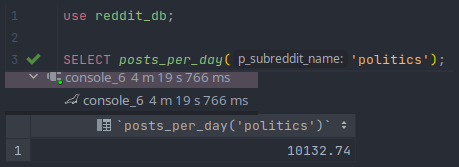
\includegraphics[width=400px] {function_avg_p_day}\label{fig:sub_ppd}
    \caption {The query was run in about 4min 20s}
\end{figure}

\subsection{How many comments include the word 'lol'}\label{subsec:how-many-comments-include}

Start by defining a procedure that stores the number of comments with the desired word in the out parameter.

\begin{verbatim}
CREATE FUNCTION posts_containing (
    p_term VARCHAR(50)
)
    RETURNS INT
    READS SQL DATA
    BEGIN
        RETURN (SELECT COUNT(*) FROM
            (SELECT * FROM test_db.comments_constrained
            WHERE body LIKE CONCAT('%', p_term, '%')) as contains_term);
    END;
\end{verbatim}

    Then it can easily be called as
    \begin{verbatim}
SELECT posts_containing ('lol');
    \end{verbatim}

The execution results are shown in figure~\ref{fig:sub_posts_containing}.

\begin{figure}[h]
    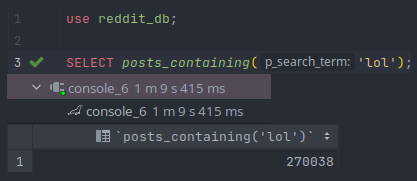
\includegraphics[width=400px] {posts_containing}\label{fig:sub_posts_containing}
    \caption {The query was run in about 1min 10s}
\end{figure}

    Whether the method should demand spaces around the search phrase is debatable.
    In the case of lol, the word is oftentimes used as one part of a longer word, so it would miss some counts there.
    On the other hand, it is likely also including some entries that wouldn't fit what the user of the procedure likely intended.

    Due to this, I think letting the caller of the method put in whitespaces themselves if they want stricter results is appropriate, and I will leave it as is.

    \subsection{Commenters of thread T have participated in what subreddits?}\label{subsec:what-subreddits}

    In MariaDB it is not possible to return multiple values from stored procedures or functions, so the stored procedure cannot return the results it found for further processing.

    \begin{verbatim}
CREATE PROCEDURE subreddits_from_link_id (
    IN p_link_id VARCHAR(10)
)
    READS SQL DATA
    BEGIN
        SELECT DISTINCT get_subreddit_name(subreddit_id) AS subreddit
         FROM test_db.comments_constrained
         WHERE author IN
               (SELECT DISTINCT author
                FROM test_db.comments_constrained
                WHERE link_id = p_link_id
                AND NOT author='[deleted]'
                );
    END;
    \end{verbatim}

    The results from me running this procedure is shown in figure~\ref{fig:subreddits_from_link} below.

\begin{figure}[h]
    
\includegraphics[width=400px] {subreddits_from_link}\label{fig:subreddits_from_link}
    \caption {The query was run in about 9s}
\end{figure}


\subsection{Which users have the highest and lowest scores?} \label{subsec:user-high-low-scores}

    These two question are basically the same, the only difference is if it is ORDER BY \ldots ASC or ORDER BY \ldots DESC.
    So I will create a view that queries the total scores of each user, and then it can be simply ordered by the total\_score column.

    Querying this view is very slow \lparen see fig~\ref{fig:user_total_score}\rparen as the GROUP BY author call is very expensive.
    It would likely be beneficial to store this as its own table to avoid having to re-compute it on every call.
    It would obviously require more storage space as what is essentially more copies of data need to be stored.
    But, considering that the computation was taking over an hour for me, it is likely worth the cost.
    Adding a trigger rule in the database that updates the values when a new value is inserted after this extra table is set up would help with keeping the database easy to use so the user won't forget updating total scores.

\begin{figure}[h]
    \includegraphics[width=400px] {TODO}\label{fig:user_total_score}
    \caption {The query was run in about 1h 20min}
\end{figure}

    \begin{verbatim}
CREATE user_total_scores AS
    SELECT author, SUM(score) AS total_score
        FROM comments_constrained
        WHERE NOT author='[deleted]'
        GROUP BY author;
    \end{verbatim}

    \subsection{Which subreddits have highest and lowest scores?} \label{subsec:subreddit-high-low-scores}
    This is basically the same as the previous question about user high scores and lowest scores, but querying for subreddits instead.
    Showing a stored procedure below.

    \begin{verbatim}
CREATE PROCEDURE subreddit_lowscores (
)
    READS SQL DATA
    BEGIN
        SELECT
        get_subreddit_name(subreddit_id) AS subreddit,
        SUM(score) AS total_score
            FROM comments_constrained
            GROUP BY subreddit
            ORDER BY total_score;
    END;
    \end{verbatim}

    \subsection{All users someone might have interacted with} \label{subsec:potential-interactions}

This means getting all links that a user has posted in, getting all comments on those links and selecting distinct authors.

    \begin{verbatim}
CREATE PROCEDURE get_interactions(
    IN p_redditor VARCHAR(20)
)
    READS SQL DATA
    BEGIN
        SELECT DISTINCT author
            FROM test_db.comments_constrained
            WHERE link_id IN
                (
                    SELECT link_id
                    FROM test_db.comments_constrained
                    WHERE author=p_redditor
                 )
            AND author NOT IN ('[deleted]', p_redditor);
    END;
    \end{verbatim}

    \subsection{All users who have only posted in one subreddit} \label{subsec:only-one-subreddit}

    This procedure gets the author and subreddit\_id columns from the comments table, and uses select distinct to
    then be able to count the number of rows grouped by author.
    Then getting those with only one subreddit is as easy as querying for where count=1.

    \begin{verbatim}
CREATE PROCEDURE only_n_subreddits(IN p_n INT)
    READS SQL DATA
    BEGIN
        SELECT *
        FROM (SELECT author, COUNT(*) AS `subreddit_count` FROM
            (SELECT DISTINCT author, subreddit_id
             FROM comments_constrained
             WHERE NOT author='[deleted]')
                AS author_reddits
              GROUP BY author) AS `only_one_reddit`
        WHERE subreddit_count<=p_n;
    END
    \end{verbatim}